\chapter{Design details}
\label{chap: dt}
The outcome of the research task previously has established clear signs for an outset of a novel bot that enables all the \textit{Evaluation Criteria} as it's features. This chapter is an explanation of the design techniques involved in building the new bot. The readers will be able to interpret the elementary idea and approach intended, concerned technologies, high-level architecture and workflow of the bot. The bot is designed to operate in Microsoft Teams. Further, it is designed in way that it can be added to multiple channels in the tool. On the whole, this Chapter gives the reader an idea of the architecture plan of D3driver and a short technology review has also been done in the end.

\section{Prerequisites}
This section describes all the terminologies needed for further understanding.
\begin{itemize}
\item Microsoft Teams\footnote{https://www.microsoft.com/en/microsoft-teams/group-chat-software} --- also called MS Teams is a well known IT collaboration tool used for communication purposes. It provides options for chat, group chats, audio and video calling, file storage and third-party apps integration. 

\item Microsoft Azure\footnote{https://docs.microsoft.com/en-us/azure/?product=featured} --- is a cloud computing platform owned by Microsoft. Users are offered a wide variety of cloud services like computing, developing, analytics, storage, networking, deploying their applications in the cloud. 

\item MS teams Adaptive cards\footnote{https://adaptivecards.io/} --- Microsoft introduced the concept of cards to exchange the UI content in a consistent way. It is a simple JSON object that can rendered within a bot. There are 3 types of cards of which adaptive cards are used for implementing the new bot. These cards can be used in bots that can either be part of bot communication or the users are also able to exchange cards with other members. There are abundant formatting options for styling the text inside the card to make it look impactful.

\item V-model --- It is the widely known and is a highly accepted model for developmental process. A team like Mechatronics that involves diverse engineering groups to build a system use this model as a guide in the different phases of development. It showcases the sequence of tasks to be carried out in each phase. The paper \cite{grassler2018v} explains the state-of-the-art theories and concepts about the model.

\end{itemize}

\section{Name and logo}
The bot is responsible for driving the whole process of Design Decision Documentation hence it is named \textbf{D3driver}, short for Design Decision Documentation driver. Presenting the logo of D3driver in \ref{fig:logonew}. The bot is aimed at successfully gathering all the design decisions made during a conversation. Accordingly, the logo exemplifies a bot that holds all the important design decision documents on one side and some more collection of the same on the other side. 
\begin{figure}[h]
\centering
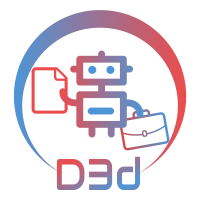
\includegraphics[width=0.6\linewidth]{figures/logonew}
\captionsetup{justification=centering}
\caption{Logo of D3driver}
\label{fig:logonew}
\end{figure}

\section{Idea and Approach}
\label{iaA}
This section is to understand the conceptual perspective of D3driver. The methodology adopted to convert each of the evaluation criterion as a functionality/feature of D3driver can be identified as follows: 
\begin{enumerate}
\item The first criterion is related to the platform of operation and D3driver is being designed and implemented in MS Teams by using all the technologies and applications that can function in MS Teams.

\item The second criterion is regarding message tagging/labeling with respect to V-model specific design phases. To this end, the bot considers the types of decisions in a mechatronics team that could possibly be discussed based on the V-model. A V-model serves as a standard for a team like mechatronics to carry out product design and development. Therefore, the bot design adheres to decision types put forward by VDI(German Association of Engineers) standards. The interpretations of V-models are explained in \cite{grassler2018v}. These globally recognized and accepted design decisions form the decision template in D3driver. The templates are designed in way that messages are tagged/labeled according to decision names defined by VDI.

\item The third criterion is the design decision management and to design this, the usage of adaptive cards in MS Teams is selected. By using adaptive cards, a clear difference can be made between common messages and important decisions.

\item The forth criterion is design decision documentation and for this purpose, the bot is designed to install a configurable tab when the bot is added to a channel. The tab is meant to display a summary of all the decisions discussed in the chat. 

\item The fifth criterion is about knowledge management and D3driver will be designed to allow users to download a copy of the decision summary that is present in the configured tab. 

\item The last criterion is about retrieving metadata from the database. D3driver will be also be designed to provide the raw data that is linked to a particular channel in the JSON format.
\end{enumerate}


Furthermore, depending on the type of V-model, the design stage in a project may be extended across different phases in a V-model.  Hence the design decisions will be discussed in all those phases and a provision to document all the decisions in all the phases is designed in D3driver. According to V-model processes in an organization, the design decisions generally could be discussed in phases like 1) Architecture design 2) Design/Concept and 3) Implementation. There are different decision types in each of these phases with regards to design and hence each phase would correspond to it’s own design decision type. In brief, the approach here is to sort the design decision types based on the respective design phases and they are as follows:
\begin{itemize}
\item Architecture design phase
\begin{enumerate}
\item Functional design hence Functional design decisions
\item Logical design hence Logical design decisions
\item Physical design hence Physical design decisions
\end{enumerate}
\item Design/Concept phase
\begin{enumerate}
\item Design definition hence Design definition decisions
\item Design characteristics \& Enablers hence Design characteristics \& Enablers decisions
\item Design Alternatives hence Design Alternatives decisions
\end{enumerate}
\item Implementation phase
\begin{enumerate}
\item Mechanical design hence Mechanical design decisions
\item Electrical design hence Electrical design decisions
\item Software design hence Software design decisions
\end{enumerate}
\end{itemize}

Each phase is designed to be a decision template in D3driver and each template will have three of it's own decision types. A new concept is introduced i.e. \textit{\textbf{Channel Initialization}}. When D3driver is added to a channel in MS Teams, that channel is supposed to be initialized with one of the decision templates. To do this, D3driver is invoked using a specific command and is only done once. After initialization, the bot is now ready to tag and document important decisions using adaptive cards. An example of adaptive card with the ``Implementation phase" and it's decision types can be viewed in \ref{fig:decisiontemplate-implementation}.

\begin{figure}
\centering
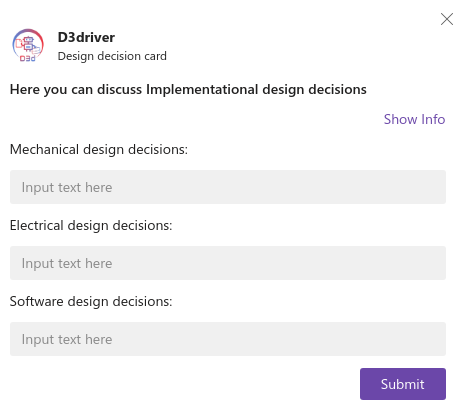
\includegraphics[width=0.7\linewidth]{figures/decisiontemplate-implementation}
\caption{Example adaptive card of Implementation phase}
\label{fig:decisiontemplate-implementation}
\end{figure}

In addition to the above design techniques, the bot is designed to use as less commands as possible to overcome the disadvantages of continuous command usage(like pointed out during the research of existing bots). The evaluation of the existing bots has also shown that in the existing designs, the users are expected to type a long and a complicated command that is a combination of many ASCII characters or the users need to make more that 2 mouse clicks to start the prioritized discussions. D3driver is designed to make the routine more effortless and thus with the help of Microsoft's \textit{Messaging Extensions}\footnote{https://docs.microsoft.com/en-us/microsoftteams/platform/messaging-extensions/what-are-messaging-extensions}, the bot adds a static button adjacent to the other default buttons beneath the standard formatting text-box. The D3driver can even be pinned to always stay visible and is just one mouse click away to start the prioritized discussions. An adaptive card will pop up as shown in the \ref{fig:decisiontemplate-implementation} upon clicking the D3driver messaging extension and further there are dedicated text-boxes to discuss prioritized messages(design decisions) whereas the other conversations that has no priority happen normally using the standard text-box offered by MS Teams. After submitting a decision to the group, all of them are stored in the database for later extraction. The D3driver tab will have a display of all the design decisions and other details like the member who took the decision, type of decision and the date of decision. A more thorough explanation of D3driver's working will be seen in the following chapter. 



\section{High-level architecture}
The figure \ref{fig:archibotnew} represents the high-level architecture of D3driver. The components of the architecture diagram are as follows:


\begin{itemize}
\item \textbf{Users} --- They symbolize the group members of a collaboration tool. The users converse with the other group members via the collaboration tool. They are the end users of D3driver. 

\item\textbf{ Collaboration tool} --- Microsoft Teams is picked as the collaboration tool for this implementation. This tool helps users to communicate with each other by means of allowing them to form teams and channels. This tool also has a rich set of conversational, productive bots that aid the users in their routine activities. This tool serves as a medium for sending and receiving messages to and from the users. Note: MS teams will come into picture once again after the bot has been hosted by Microsoft Azure. Teams is responsible for creating an important file along with logo icon-files to finally use the bot. This details of which will be discussed in the implementation chapter.

\item \textbf{Channel connector} --- A connection link between the Microsoft teams and D3driver is none other than the channel connector. To be able to deploy D3driver in the bot studio of MS teams, one must register it with Microsoft Azure bot service. Microsoft Azure has a set of approved channels. The developer must set the bot up with the appropriate channel available in Microsoft Azure. In this case, the bot should be configured with Microsoft Teams. This means the D3driver will be able to talk to users via Microsoft Teams. This connector is responsible for forwarding user’s incoming messages to the bot’s endpoint appended with the standard endpoint of MS Teams i.e. \textbf{/api/messages}. Here is an official documentation\footnote{https://docs.microsoft.com/en-us/azure/bot-service/bot-service-manage-channels?view=azure-bot-service-4.0} on how to structure bots with channels with the help of Microsoft Azure

\begin{figure}[h]
\centering
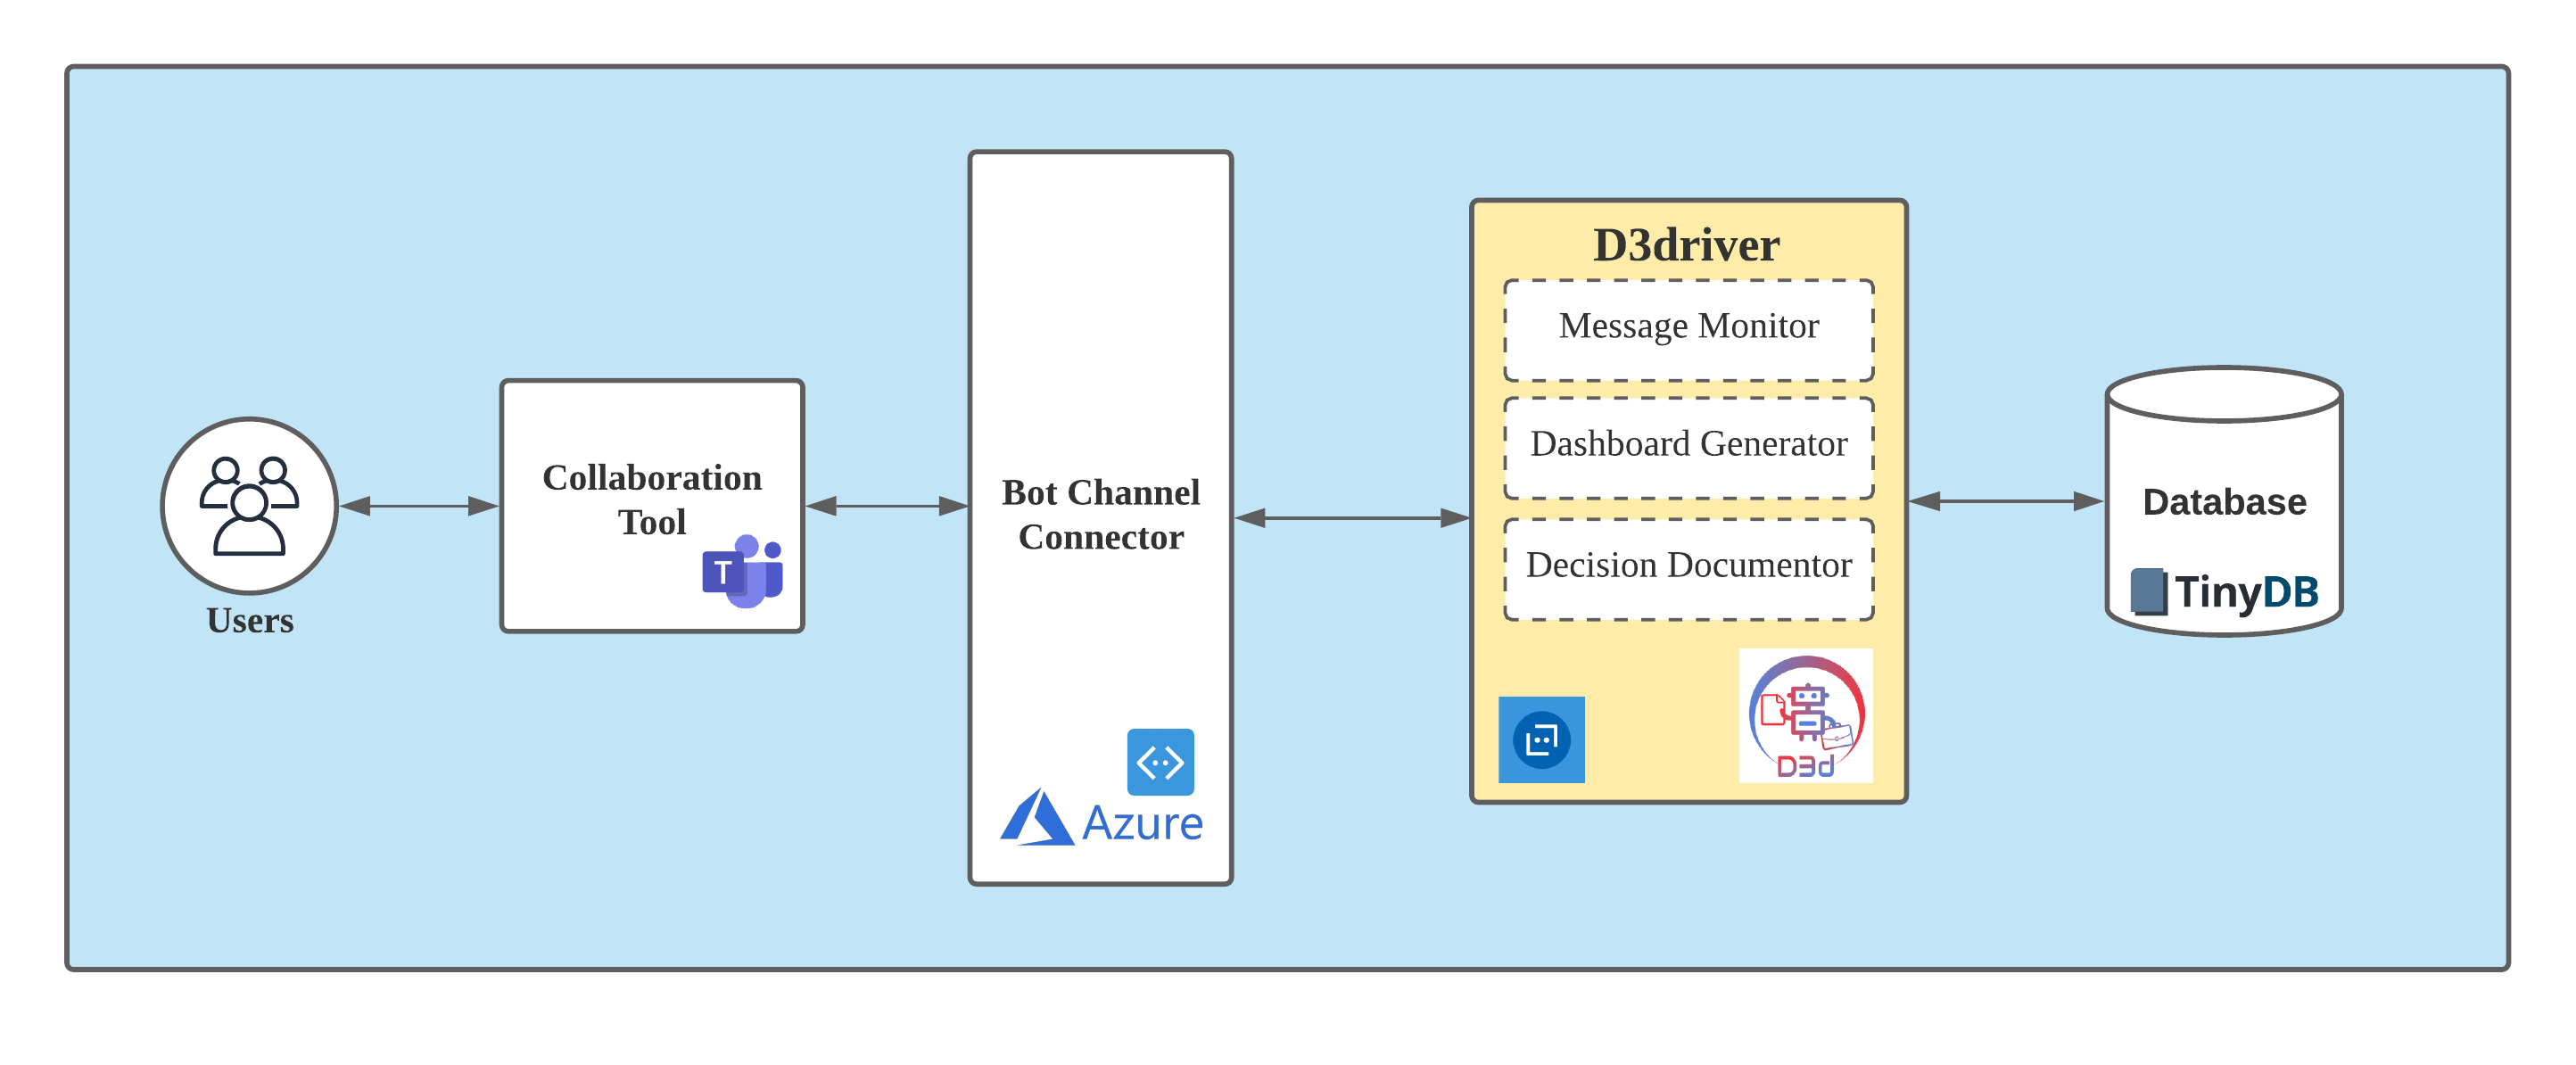
\includegraphics[width=1.1\linewidth]{figures/archibotnew}
\captionsetup{justification=centering}
\caption{ High-level bot architecture}
\label{fig:archibotnew}
\end{figure}


\item  \textbf{Bot Framework v4} --- Azure Bot Service offers a complete toolkit required to build bots, for example the popular Bot framework SDK. This framework is the core of D3driver and is the main element for developing any MS Teams bot. The framework provides many schema and this implementation will use cards schema. Card schema is the representation of interactive adaptive cards in the application-level, that can be used inside a group chat. After the bot development, the developer is required to create a new bot service by providing all the desired data. Information like name of the bot, developer location, Bot template(v4), Bot ID and password etc should all be mentioned during the registration. This will help Azure to create the bot service and deploy the bot to the cloud. After successful deployment, the developer will prepare all the necessary code files to deploy. All the files should be zipped up i.e, the python files(app.py), dependency files(requirement.txt) etc. The deployment and the channel connector configurations should make the bot available inside MS teams bot studio. Once again the official documentation for this can be seen here\footnote{https://docs.microsoft.com/en-us/azure/bot-service/abs-quickstart?view=azure-bot-service-4.0}

\item \textbf{Database} --- This is the storage component in the architecture. This serves as the persistence layer for D3driver. The incoming decisions should be stored for later retrieval and hence it would require a simple database for that purpose. TinyDB is written in python and can be easily extended to make use of custom storage. The main function of the database is to store the details like channel name, sender’s name, decision name and date etc. It can be devised to store any schema that a developer would design. After storing, it can be queried to display any data the developer wants to display on the D3driver tab.

\end{itemize}



\section{Work-flow of D3driver}

This section describes the step-by-step working of the D3driver by means of a flowchart as shown in figure \ref{fig:d3dflowchartpng}. The flowcharts depicted has 3 parts. The left hand side of the flowchart denotes the main working procedure of the D3driver using messaging extension. The central part of the flowchart depicts the process of channel initialization and the right hand side of the flowchart depicts the operations that can be performed in the D3driver tab. As soon as D3driver is installed to a channel in MS Teams, two processes will take place. 1) the D3driver's Messaging Extension will be installed and 2) D3driver's Configurable Tab will be installed. The channel initialization is done by invoking the D3driver. The bot will post a card where it asks the users to choose from one of the V-model phases. Any user selects a suitable V-model phase which is required according to their project. After selection, appropriate messages will be posted by D3driver in the group like which V-model phase has been selected and the name of the user who made this choice. 

After a V-model process is selected, the D3driver’s messaging extension(button) can be clicked to start a conversation related to design decisions. Upon clicking, an adaptive card pops up with three other input fields and their names are dependent on the V-model phase chosen for the team/project during channel initialization. The user can make use of those intended fields to discuss design decisions. After a decision is typed, the users can click on the ``submit button" within the card. Upon clicking the submit button, the typed decision is posted into the channel window. The typed decision also appears in the form of a card with name of the decision type, name of the decision maker, date of decision and the actual decision itself. This way, all design decisions are sorted from the other normal conversation material in the group chat. All these cards are saved into the D3driver's database.

The right most part of the flowchart denotes the visualization of all the saved decisions. The purpose of having a D3driver tab is to display all the decisions in one place. After the decision cards were exchanged, all the information is saved to the database and is rendered as a HTML page on the D3driver tab. The work flow of this is also simple. Any user who wants to take a look at all the decisions that has been discussed can click on the designated D3driver tab of a channel(There will be separate D3driver tabs for different channels and will contain the information that is regarded to the respective channel only). In the tab, a dashboard can be viewed with the type of channel initialization, decision type, date, decision maker etc. A search box functionality is designed to filter the desired decision card. A sort button functionality is designed to sort the decisions according to the date. A button that allows the users to download a copy of all the information present in the tab is designed. Finally, a button to view the metadata of that channel's decision cards is designed.

\begin{figure}
\centering
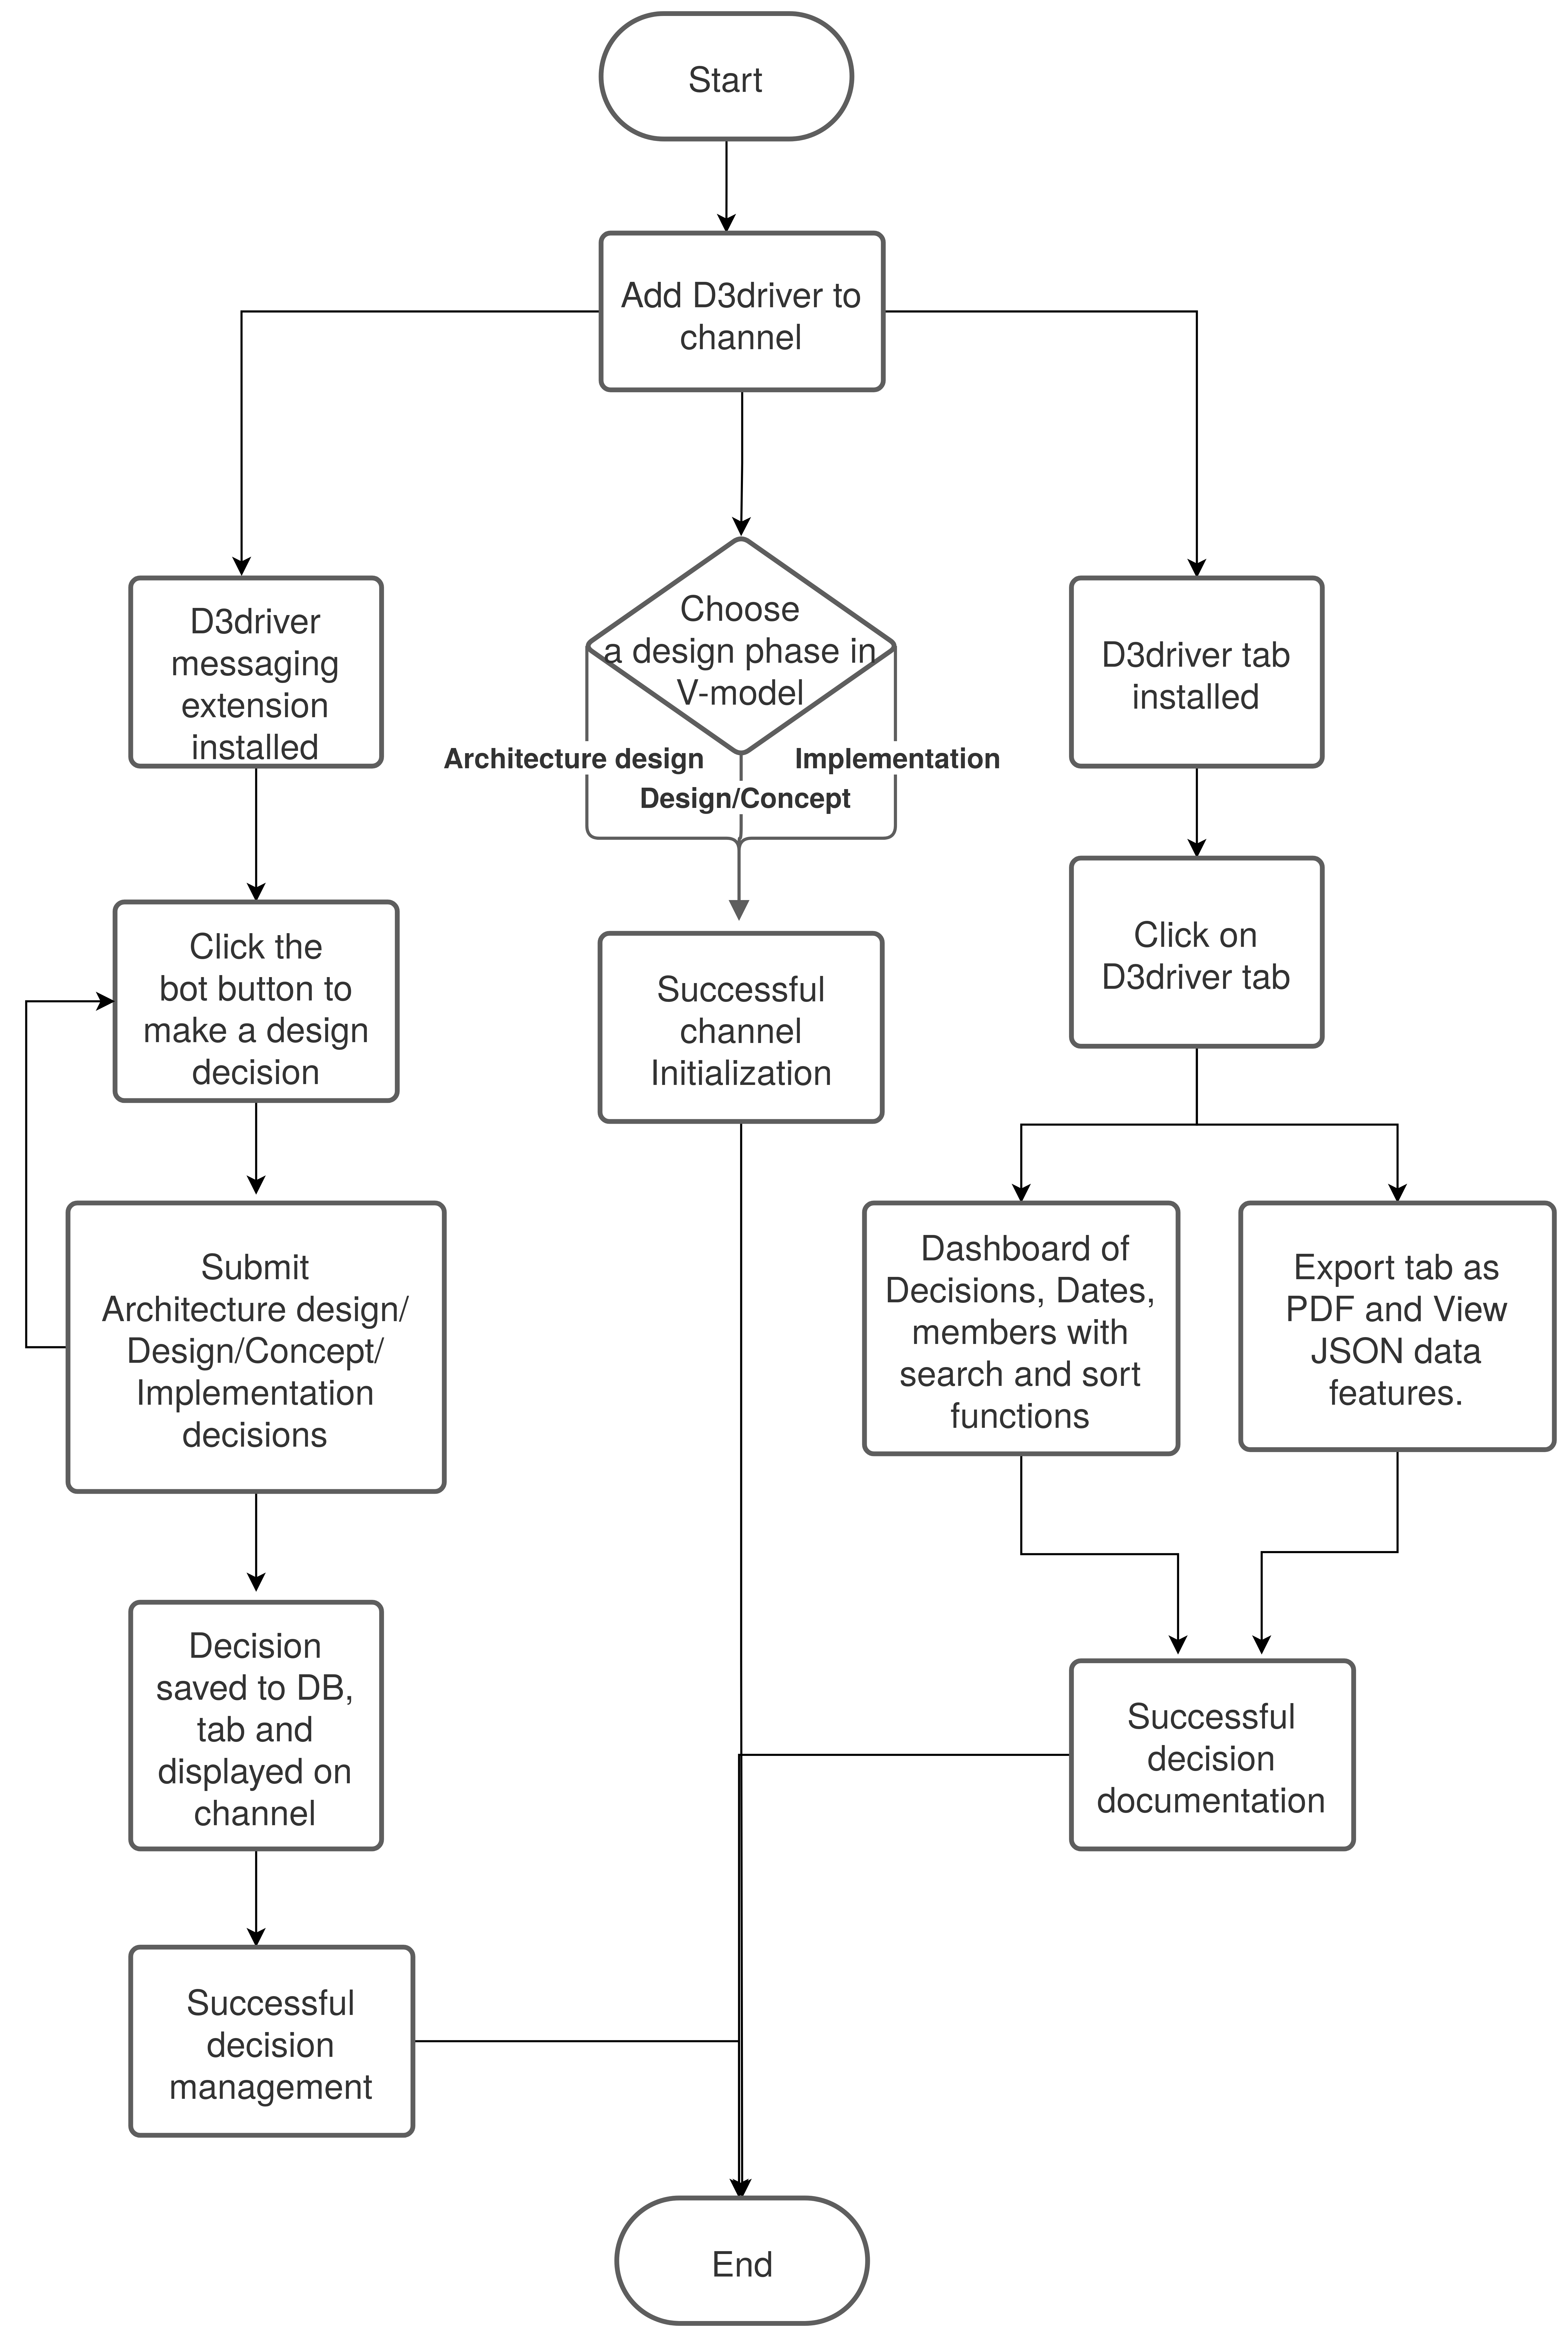
\includegraphics[width=1\linewidth]{figures/d3dflowchartpng}
\caption{Workflow of D3driver}
\label{fig:d3dflowchartpng}
\end{figure}


\section{Technologies and Applications}

The choice of technologies and applications that will be used for the implementation are listed in this section:

\begin{itemize}
\item  Microsoft Teams --- The D3driver app package is designed and developed in such a way that it can be integrated to any collaboration tool but this thesis implementation focuses on hosting the bot in Microsoft teams hence this app is the obvious choice.

\item  Microsoft Azure --- This cloud service seems to be the best to work with Microsoft teams and also the platform ensures a great collection of bot framework features. The open-source bot framework SDK v4 is an ideal development toolkit for this implementation.

\item ngrok\footnote{https://ngrok.com/docs} --- is a tunneling tool that helps users to expose their local-host server to the internet. This is a free software that can be downloaded on the system. ngrok uses either the default HTTP port or an explicit port number can be mentioned such that ngrok exposes that local port.

\item Python SDK version 3.7\footnote{https://www.python.org/} --- One of the popular programming languages that makes use of an interpreter making it an interpreted, high-level language. This is used as the main developing language for D3driver because it has simpler syntax, easy usage, can be executed faster and works well for prototyping software.

\item TinyDB\footnote{https://tinydb.readthedocs.io/en/latest/} --- As discussed in the architecture plan, this database will be used as decision database for D3driver. The design of the database is that it will have two tables to store channel related information and decision related information.

\item  HTML\footnote{https://www.w3.org/TR/html52/} \& JavaScript\footnote{https://devdocs.io/javascript/} --- D3driver tab uses these two technologies to render the card summary and other details. HTML to display the card information and JavaScript to make the page interactive.

\item  Visual studio code\footnote{https://code.visualstudio.com/} --- This is the best code editor created by Microsoft. Excellent features for code debugging, code review integrated with version control system(github). The biggest advantage is the availability of "Microsoft UI toolkit" extension with visual studio code specially used for bot development and management. It has some internal configurations with Azure that is done automatically for users and makes the process easier and faster.
\end{itemize}


This design is supposed to be the solution to poor or no documentation in a multi-disciplinary team. The design of D3driver aims at motivating team members to distinguish the most important design decisions from the typical conversations that they would have among their team. Designed in the best possible way to balance the simplicity, usability and functionality of the bot. The design also exhibits flexibility to choose the type of V-model process standard that the team wants to document. The design in ease of using the card with just one click is also the highlight and finally a dedicated tab to persist all the decisions together shows that the design is meant to decrease any effort of going through
the long threads of decisions in a channel.













